\part{Teoria della complessità}
\chapter{Complessità di tempo}
Anche quando un problema è decidibile, e quindi in linea di principio computazionalmente risolvibile, può non essere risolvibile in pratica se la soluzione richiede una quantità eccessiva di tempo o di memoria. In questa parte introduciamo la teoria della complessità computazionale, uno studio del tempo, della memoria o di altre risorse necessarie per risolvere problemi computazionali.

\section{Misure di complessità}
Per semplicità si calcola il tempo di esecuzione di un algoritmo semplicemente in funzione della lunghezza della stringa che rappresenta l'input e non si considerano eventuali altri parametri. Nell'analisi del caso peggiore, che noi considereremo, si valuta il tempo di esecuzione massimo tra tutti gli input di una determinata lunghezza. Nell'analisi del caso medio, si considera la media dei tempi di esecuzione su tutti gli input di una determinata lunghezza.

\begin{Definition}{Complessità temporale di una TM}{}
Sia $M$ una macchina di Turing deterministica che si ferma su tutti gli input. Il tempo di esecuzione o la complessità di tempo di $M$ è la funzione $f: \mathbb{N}\longrightarrow\mathbb{N}$ dove $f(n)$ è il numero massimo di passi che $M$ utilizza su un qualsiasi input di lunghezza $n$.  
\end{Definition}

Ad esempio sia $M$ il decisore definito come:

\textit{M = "Data la stringa w in input:}
\begin{enumerate}
    \item Muovi la testina a destra finché non viene letto il simbolo $\sqcup$
    \item Accetta"
\end{enumerate}
Data in input una stringa $w$ tale che $|w| = n$, la TM $M$ impiega $n$ passi. Di conseguenza, il suo tempo computazionale è $f(n) = n$.

\subsection{Notazione O-grande ed o-piccola}
Poiché il tempo esatto di esecuzione di un algoritmo è spesso un'espressione complessa, solitamente ci limitiamo ad ottenerne una stima. Il metodo di stima, detto analisi asintotica, permette di valutare il tempo di esecuzione dell'algoritmo quando viene eseguito su grandi input. Lo facciamo prendendo in considerazione solo il termine di ordine maggiore dell'espressione del tempo di esecuzione dell'algoritmo, trascurando sia il coefficiente di tale termine, che tutti i termini di ordine inferiore, perché il termine di ordine più alto domina gli altri termini quando l'input è grande.

\begin{Definition}{O-grande}{}
Siano $f$ e $g$ funzioni $f,g: \mathbb{N}\longrightarrow\mathbb{R}^+$. Si dice che $f(n) = O(g(n))$ se esistono interi positivi $c$ e $n_0$ tali che per ogni $n \geq n_{0}$,
\begin{equation*}
    f(n) \leq cg(n)    
\end{equation*}
Quando $f(n) = O(g(n))$ diciamo che $g(n)$ è un limite superiore asintotico per $f(n)$.
\end{Definition}

\begin{Definition}{o-piccolo}{}
Siano $f$ e $g$ funzioni $f ,g: \mathbb{N}\longrightarrow\mathbb{R}^+$. Diciamo che $f(n) = o(g(n))$ se 
\begin{equation*}
\lim_{n\to\infty}\frac{(f(n))}{g(n)}=0
\end{equation*}
In altri termini, $f(n) = o(g(n))$ significa che per ogni numero reale $c > 0$ esiste un numero $n_0$, tale che $f(n) < cg(n)$ per ogni $n \geq n_{0}$.
\end{Definition}

\begin{Example}{Rapporto di tempo tra TM multinastro e TM}{}
\textit{Sia $t(n)$ una funzione tale che $t(n) \geq n$. Per ogni TM multinastro $M$ con tempo $t(n)$ esiste una TM $M'$ tale che $L(M) = L(M')$ avente tempo $O(t^2(n))$.}

Consideriamo la TM $S$ in grado di simulare una TM multinastro. Analizziamo quindi la complessità temporale di $S$:
\begin{enumerate}
    \item Il numero di nastri $k$ è indipendente dall’input.
    \item Per preparare il nastro sono necessari $kO(n) = O(n)$ passi.
    \item Per ogni passo simulato della TM multinastro, $S$ richiede $kO(t(n)) = O(t(n))$ passi.
    \item Il numero di passi della TM multinastro è $t(n)$.
\end{enumerate}
Di conseguenza, la complessità temporale di $S$ risulta essere: 
\begin{equation*}
    t'(n) = O(n) + t(n)O(t(n)) = O(n) + O(t^2(n)) = O(t^2(n))
\end{equation*}
\end{Example}

\begin{Definition}{Complessità temporale di una NTM}{}
Sia $N$ un decisore non-deterministico. Definiamo come complessità temporale di $N$
la funzione $f : \mathbb{N}\to \mathbb{N}$ tale che $f(n)$ sia il massimo numero di passi necessari ad ogni ramo dell’esecuzione di $D$ per processare una stringa di lunghezza $n$.
\end{Definition}

\begin{Example}{Rapporto di tempo tra NTM e TM}{}
\textit{Sia $t(n)$ una funzione tale che $t(n) \geq n$. Per ogni NTM $N$ con tempo $t(n)$ esiste una
TM $M'$ tale che $L(M) = L(M')$ avente tempo $2^{O(t(n))}$.}

Consideriamo la TM $M$ in grado di simulare una NTM. Analizziamo quindi la complessità temporale di $M$:
\begin{enumerate}
    \item Il numero massimo $b$ di figli di ogni nodo è indipendente dall’input.
    \item Di conseguenza, il numero di foglie dell’albero computazionale risulta essere $k \leq b^{t(n)}$, implicando che il numero massimo di nodi sia $m\leq 2b^{t(n)}$, dunque $m = O(b^{t(n)})$.
    \item $M$ simula ogni nodo dell’albero computazionale ripartendo sempre dalla radice, dunque esegue $O(t(n)b^{t(n)})$ passi.
\end{enumerate}
A questo punto, notiamo che:
\begin{equation*}
t(n)b^{t(n)} = 2{\log_2(t(n)b^{t(n)})} = 2^{\log_2(t(n))+t(n)\log_2b} = 2^{O(t(n))}
\end{equation*}
Di conseguenza, la complessità temporale di M risulta essere:
\begin{equation*}
t'(n) = O(t(n)b^{t(n)}) = O(2^{O(t(n))}) = 2^{O(t(n))}
\end{equation*}
\end{Example}

\section{Classe P}
\begin{Definition}{Classe DTIME}{}
Data la funzione $t :\mathbb{N}\to \mathbb{R}^+$, definiamo come classe dei linguaggi decidibili in tempo $O(t(n))$ il seguente insieme:
\begin{equation*}
    DTIME(t(n)) = \{L\in DEC | L\textit{ decidibile da una }TM\textit{ in tempo }O(t(n))\}
\end{equation*}
\end{Definition}

\begin{Definition}{Classe P}{}
$P$ è la classe di linguaggi che sono decidibili in tempo polinomiale su una macchina di Turing deterministica a singolo nastro. In altre parole,
\begin{equation*}
P = \bigcup_k DTIME(n^k)    
\end{equation*}
\end{Definition}

La classe $P$ ha un ruolo centrale nella nostra teoria ed è importante perché è una classe matematicamente robusta rispetto alle varianti di TM che abbiamo studiato.

\begin{Definition}{Classe EXP}{}
Definiamo la classe dei linguaggi decidibili in tempo esponenziale come:
\begin{equation*}
EXP = \bigcup_{k\in\mathbb{N}}DTIME(2^{n^k})
\end{equation*}

Ovviamente $P\subseteq EXP$ e $P\neq EXP$.
\end{Definition}

\begin{Example}{Problema dei cammini}{}
\textit{Un grafo orientato $G$ contiene nodi $s$ e $t$. Il problema $PATH$ consiste nel determinare, se esiste, un cammino diretto $s$ a $t$.}

Sia $PATH =\{(G,s,t)| G\textit{ è un grafo orientato che contiene un cammino diretto da }s\textit{ a }t\}$.

Dobbiamo dimostrare se $PATH$ è polinomialmente decidibile, ossia $PATH\in P$.
\begin{osservation}
Dimostriamo questo teorema presentando un algoritmo di tempo polinomiale che decide $PATH$. Un potenziale cammino è una sequenza di nodi in $G$ avente lunghezza al più $m$, dove $m$ è il numero di nodi in $G$. (Se esiste un qualche cammino diretto da $s$ a $t$, ne deve esistere necessariamente almeno uno avente lunghezza al massimo $m$, perché non è mai necessario ripetere un nodo.)

Per ottenere un algoritmo polinomiale per $PATH$, si può utilizzare un metodo visita dei grafi come la visita in ampiezza. In questo caso, contrassegniamo successivamente tutti nodi in $G$ che sono raggiungibili da $s$ mediante cammini diretti di lunghezza 1, poi 2, poi 3, fino ad $m$.    
\end{osservation}
\begin{demonstration}
Un algoritmo in tempo polinomiale M per PATH funziona come segue.

$M=$ "Su input $(G, s,t)$, dove $G$ è un grafo orientato con nodi $s$ e $t$:
\begin{enumerate}
    \item Marca il nodo $s$.
    \item Ripete il seguente passo fino a quando nessun nuovo nodo viene marcato:
    \begin{enumerate}
        \item Scansiona tutti gli archi di $G$. Se trova un arco $(a, b)$ che va da un nodo $a$ marcato ad un nodo $b$ non marcato, marca il nodo $b$.
    \end{enumerate}
    \item Se $t$ è marcato, accetta. Altrimenti, rifiuta."
\end{enumerate}
Ora analizziamo questo algoritmo per dimostrare che lavora in tempo polinomiale. Ovviamente, le fasi 1 e 3 sono eseguite una sola volta. La fase 2 è eseguita al più $m$ volte perché ogni volta, tranne l'ultima, marca un nodo aggiuntivo in $G$. Quindi il numero totale di fasi utilizzate è al massimo $1+1+m$, che da un polinomio nella dimensione di $G$.    
\end{demonstration}
\end{Example}

\section{Classe NP}
\begin{Definition}{Classe NTIME}{}
Data la funzione $t : \mathbb{N}\to\mathbb{R}^+$, definiamo come classe dei linguaggi decidibili non-deterministicamente in tempo $O(t(n))$ il seguente insieme:
\begin{equation*}
    NTIME(t(n)) = \{L\in DEC | L\textit{ decidibile da una NTM in tempo }O(t(n))\}
\end{equation*}
\end{Definition}

\begin{Definition}{Verificatore}{}
Un verificatore per un linguaggio $A$ è un algoritmo $V$, dove
\begin{equation*}
    A=\{w|V\textit{ accetta }\langle w, c\rangle\textit{ per qualche stringa }c\}
\end{equation*}
dove la stringa c viene detta certificato di appartenenza. Misuriamo il tempo di un verificatore solo in termini della lunghezza di $w$, quindi un verificatore in tempo polinomiale viene eseguito in tempo polinomiale nella lunghezza di $w$. Un linguaggio $A$ è polinomialmente verificabile se ammette un verificatore in tempo polinomiale.
\end{Definition}

\begin{Definition}{Classi NP e NEXP}{}
Definiamo la classe dei linguaggi decidibili non-deterministicamente in tempo polinomiale come:
\begin{equation*}
NP = \bigcup^\infty_{k=1}NTIME(n^k)
\end{equation*}
oppure si può definire NP come la classe dei linguaggi che ammettono un verificatore in tempo polinomiale.

Analogamente, definiamo la classe dei linguaggi decidibili non-deterministicamente in tempo esponenziale come:
\begin{equation*}
NEXP = \bigcup^\infty_{k=1}NTIME(2^{n^k})
\end{equation*}
\end{Definition}

\begin{Corollario}{Gerarchia temporale dei linguaggi}{}\label{cor:gerarchia-temp-ling}
\textit{Date le classi $P$, $NP$ e $EXP$, si ha che:}
\begin{equation*}
    P \subseteq NP \subseteq EXP \subseteq NEXP
\end{equation*}
\begin{demonstration}
Per definizione stessa, una TM risulta essere anche una NTM. Di conseguenza, ne segue automaticamente che $P \subseteq NP$ e che $EXP \subseteq NEXP$. Inoltre, per il corollario precedente, abbiamo che:
\begin{equation*}
    L \in NP\implies \exists k \in N | L \in NTIME(n^k)\implies L \in DTIME(2^{O(n^k)})\implies L \in EXP
\end{equation*}
\end{demonstration}
\end{Corollario}

\begin{Definition}{CLIQUE}{}
Definiamo come $CLIQUE$ il seguente linguaggio: 
\begin{equation*}
    CLIQUE = \{\langle G, k\rangle | G\textit{ grafo non diretto con una }k\textit{-clique}\}
\end{equation*}
dove una $k$-clique è un sottoinsieme di nodi dove ognuno di quest'ultimi è adiacente a tutti gli altri nodi del sottoinsieme.

Ovvero una clique, in un grafo non orientato, è un sottografo in cui ogni due nodi sono collegati da un arco. Una $k$-clique è una clique che contiene $k$ nodi.
\end{Definition}

\begin{Example}{Problema della tricolorazione dei grafi}{}
Definiamo il linguaggio del problema della tricolorazione dei grafi come:
\begin{equation*}
    3COL = \{\langle G\rangle | G = (V_G, E_G)\textit{ grafo 3-colorabile}\}
\end{equation*}
dove un grafo è detto 3-colorabile se ad ogni suo nodo è possibile assegnare un colore diverso dai suoi nodi adiacenti utilizzando al massimo tre colori.

Vogliamo dimostrare se $3COL$ è polinomialmente verificabile ovvero $3COL\in NP$.
\begin{demonstration}
Sia $V$ la TM definita come:

$V =$ "Data la stringa $\langle \langle G\rangle, c\rangle$ in input, dove $G = (V_G, E_G)$ è un grafo:
\begin{enumerate}
    \item Interpreta $c$ come $c = \langle c_1,...,c_m\rangle$, dove $m = |V_G|$ e $\forall k \in [1, m]$, $c_k \in \{R, G, B\}$.
    \item Ripeti lo step successivo per ogni arco $(v_i, v_j) \in E_G$:
    \begin{enumerate}
        \item Se $c_i = c_j$, allora rifiuta.
    \end{enumerate}
    \item Accetta"
\end{enumerate}
Per costruzione stessa di $V$, si ha che:
\begin{align*}
\langle G\rangle \in 3COL \iff\textit{ Esiste una colorazione valida }c_1,...,c_n\\\iff \exists c = \langle c_1,...,c_n\rangle \in \Sigma^*,\langle \langle G\rangle, c\rangle \in V
\end{align*}
dunque $V$ risulta essere un verificatore di $3COL$. Analizziamo quindi il costo di $V$:
\begin{enumerate}
    \item La prima istruzione è eseguibile in $O(|w|) = O(n)$.
    \item La seconda istruzione è eseguibile in $O(n^k)$ per qualche $k \in N$.
    \item Il ciclo viene eseguito per $O(|E_G|) = O(m^2) = O(n^2)$ iterazioni, dove ognuna di quest’ultime richiede $O(1)$.
\end{enumerate}
Di conseguenza il costo computazione di V risulta essere:
\begin{equation*}
    t(n) = O(n) + O(n^k) + O(n^2)O(1) = O(n^k)
\end{equation*}
implicando che $V$ sia un verificatore polinomiale e quindi che $3COL \in NP$.
\end{demonstration}
\end{Example}

\begin{Thm}{Classe NP (definizione alternativa)}{}
\textit{Data la classe $NP$, si ha che $NP = \{L \in DEC | \exists V\textit{ verificatore polinomiale per }L\}$.}

In altre parole, possiamo definire NP anche come la classe dei linguaggi verificabili
in tempo polinomiale.

\begin{demonstration}
Dato $L\in NP$, sia $N$ la NTM tale che $L = L(N)$. Durante la sua computazione, $N$ effettuerà una serie di scelte, creando così il suo albero di computazione. Sia $V$ la TM definita come:

$V =$ "Data la stringa $\langle w, c\rangle$ in input:
\begin{enumerate}
    \item Interpreta $c$ come una serie di scelte da effettuare
    \item Simula $N$ su input $w$ eseguendo le scelte dettate da $c$
    \item Se la simulazione accetta, $V$ accetta. Altrimenti, rifiuta"
\end{enumerate}
Per costruzione stessa di $V$, si ha che:
\begin{align*}
w \in L = L(N) \iff\textit{ Esiste un ramo di }N \textit{ che accetta }w \iff \exists c \in \Sigma^*,\langle w, c\rangle \in L(V)
\end{align*}
dunque $V$ risulta essere un verificatore di $L = L(N)$. Inoltre, poiché $L = L(N) \in NP$, la lunghezza massima dei rami dell’albero di computazione risulta essere $O(n^k)$. Di conseguenza, ogni certificato può avere al massimo $O(n^k)$ scelte, implicando che $V$ sia un verificatore polinomiale.

Dato un linguaggio $L$, supponiamo che esista un verificatore $V$ che verifica $L$ in tempo polinomiale, implicando che:
\begin{equation*}
    \exists k \in N | V\textit{ verifica }L\textit{ in }O(n^k)
\end{equation*}
Sia $N$ la NTM definita come: 

$N =$ "Data la stringa $\langle w\rangle$ in input:
\begin{enumerate}
    \item Scegli non deterministicamente una stringa $c$ di lunghezza $O(n^k)$.
    \item Simula $V$ su input $\langle w, c\rangle$.
    \item Se la simulazione accetta, $B$ accetta. Altrimenti, rifiuta"
\end{enumerate}
Essendo $N$ una NTM, l’esecuzione del primo passo genererà un albero computazionale in cui ogni ramo analizza una sola tra tutte le possibili stringhe di lunghezza $O(n^k)$. In particolare, almeno uno di questi rami analizzerà un certificato valido. Di conseguenza, si ha che:
\begin{align*}
w \in L \iff \exists c \in \Sigma^*,\langle w, c\rangle \in V \iff\textit{ Esiste un ramo di }N\textit{ che accetta }w \iff x \in L
\end{align*}
implicando che $L \in L(N) \in NP$.
\end{demonstration}
\end{Thm}

\section{NP-completezza}
\begin{Definition}{Funzione calcolabile in tempo polinomiale}{}
Una funzione $f:\Sigma^*\to\Sigma^*$ è una funzione calcolabile in tempo polinomiale se esiste una macchina di Turing di tempo polinomiale $M$ che si arresta con $f(w)$ soltanto sul suo nastro, quando ha iniziato con un qualsiasi input $u$.    
\end{Definition}

\begin{Definition}{Riducibile in tempo polinomiale}{}
Il linguaggio $A$ è riducibile mediante funzione in tempo polinomiale, o semplicemente riducibile in tempo polinomiale, al linguaggio $B$, denotato con $A \leq_P B$ se esiste una funzione calcolabile in tempo polinomiale $f : \Sigma^*\longrightarrow\Sigma^*$ dove, per ogni $w$,
\begin{equation*}
    w \in A \iff f(w) \in B    
\end{equation*}
La funzione $f$ è chiamata riduzione di tempo polinomiale di $A$ a $B$.
\end{Definition}

\begin{Example}{Problema della soddisfacibilità delle 3CNF}{}
\textit{Definiamo il linguaggio del problema della soddisfacibilità delle $3CNF$ come:}
\begin{equation*}
    3SAT = \{\langle \phi\rangle | \phi\textit{ è una }3CNF\textit{ soddisfacibile}\}
\end{equation*}
dove una $3CNF$ è una formula logica formata da un $and$ logico tra $n$ clausole, ciascuna
formata da un $or$ logico tra 3 letterali, ossia una variabile negata o non. La seguente formula è una 3CNF:
\begin{equation*}
    (x_1 \lor \overline{x_2} \lor \overline{x_3}) \land (x_3 \lor \overline{x_5} \lor x_6) \land (x_3 \lor \overline{x_6} \lor x_4) \land (x_4 \lor x_5 \lor x_6)
\end{equation*}
Inoltre, tale formula è soddisfacibile dal seguente assegnamento:
\begin{equation*}
    x_1 = 1, x_2 = 0, x_3 = 1, x_4 = 1, x_5 = 1, x_6 = 0    
\end{equation*}
\end{Example}

\begin{Thm}{3SAT riducibile in tempo polinomiale a CLIQUE}{}
\textit{$3SAT$ è riducibile in tempo polinomiale a $CLIQUE$.}
\begin{osservation}
La riduzione di tempo polinomiale $f$ che mostriamo di $3SAT$ a $CLIQUE$ converte formule in grafi. Nei grafi costruiti, clique di una dimensione specificata corrispondono ad assegnamenti soddisfacenti per la formula. Le strutture all'interno del grafo sono progettate per simulare il comportamento delle variabili e delle clausole.
\end{osservation}
\begin{demonstration}
Sia $f : \Sigma^*\longrightarrow\Sigma^*$ la funzione calcolata dalla seguente TM $F$ definita come:

$F =$ "Data la stringa $\langle\phi\rangle$ in input:
\begin{enumerate}
    \item Costruisci un grafo $G$ definito come:
    \begin{enumerate}
        \item Conta il numero $k$ di clausole $or$ in $\phi$.
        \item Per ogni clausola, crea un nodo $x_i$ per ogni letterale della clausola, creando dei doppioni se il letterale compare più volte.
        \item Organizza i nodi di $G$ in $k$-triple (una per clausola $or$), dove tre nodi appartengono alla stessa tripla se e solo se i loro letterali compaiono all’interno di una stessa clausola $or$.
        \item Crea un arco tra ogni coppia di nodi fatta eccezione di nodi appartenenti alla stessa tripla e nodi rappresentanti letterali opposti tra loro (es: $x_i$ e $\overline{x_i}$).
    \end{enumerate}
    \item Restituisci in output la stringa $\langle G, k\rangle"$
\end{enumerate}

\begin{minipage}{\textwidth}
    \centering
    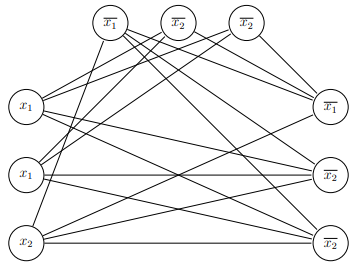
\includegraphics[width=0.5\textwidth]{images/3sat-clique.PNG}
    \captionof{figure}{Grafo generato dalla funzione f della dimostrazione a partire dalla formula $\phi = (x_1 \lor x_1 \lor x_2) \land (x_1 \lor x_2 \lor x_2) \land (x_1 \lor x_2 \lor x_2)$}
\end{minipage}

Supponiamo che $\langle\phi\rangle\in 3SAT$. Poiché $\phi$ è una $3CNF$, affinché essa sia soddisfacibile ne segue che ogni clausola sia soddisfacibile, dunque che almeno uno dei letterali di ognuna di tali clausole sia vero. Sia quindi $C = \{x_1, . . . , x_k\}$ l’insieme dei nodi tali che $\forall i\in [1, k]$, $x_i$ è il nodo corrispondente al letterale vero della $i$-esima tripla. Poiché tali nodi appartengono tutti a triple diverse e poiché $\nexists x_i, xj\in C$ tali che $x_i = x_j$ in quanto non possono essere entrambi veri, ne segue che essi siano tutti due a due adiacenti, implicando che $C$ sia una $k$-clique. Di conseguenza, abbiamo che:
\begin{equation*}
    \langle\phi\rangle\in 3SAT \implies f(\langle\phi\rangle) = \langle G, k\rangle \in CLIQUE
\end{equation*}
Supponiamo ora che $f(\phi) = \langle G, k\rangle \in CLIQUE$, implicando che esista una $k$-clique al suo interno. Dunque, per costruzione di $G$, non esistono nodi all’interno della
clique i cui letterali rappresentati appartengono alla stessa tripla. A questo punto, poiché tali letterali non interferiscono tra loro trovandosi in triple diverse, esiste un assegnamento che soddisfi ogni clausola. In particolare, tale assegnamento risulta sempre possibile in quanto all’interno della clique non possano appartenere sia $x_i$ che $\overline{x_i}$. Di conseguenza, abbiamo che:
\begin{equation*}
    f(\langle \phi\rangle) = \langle G, k\rangle \in CLIQUE \implies \langle \phi\rangle \in 3SAT   
\end{equation*}
implicando quindi che:
\begin{equation*}
    \langle \phi\rangle \in 3SAT \iff f(\langle \phi\rangle) = \langle G, k\rangle \in CLIQUE
\end{equation*}
Inoltre, poiché $F$ svolge solo operazioni eseguibili in tempo polinomiale, concludiamo
che $3SAT \leq^P_m CLIQUE$.
\end{demonstration}
\end{Thm}

\subsection{Riducibilità in tempo polinomiale}
\begin{Definition}{Riducibilità in tempo polinomiale}{}
Dati due linguaggi $A$ e $B$, diciamo che $A$ è riducibile in tempo polinomiale a $B$ tramite mappatura, indicato come $A \leq^P_m B$, se esiste una funzione calcolabile $f : \Sigma^*\to \Sigma^*$, detta riduzione in tempo polinomiale da $A$ a $B$, tale che:
\begin{equation*}
    w\in A\iff f(w)\in B
\end{equation*}
e $f$ è calcolabile in tempo polinomiale.
\end{Definition}

\begin{Thm}{ Decidibilità polinomiale tramite riduzione}{}
Dati due linguaggi $A$ e $B$ tali che $A \leq^P_m B$, si ha che:
\begin{equation*}
    B\in P\implies A\in P
\end{equation*}

\begin{demonstration}
Dato $B\in P$, sia $DB$ il decisore tale che $L(DB) = B$. Sia $DA$ la TM definita come:

$DA =$ "Data la stringa $w$ in input:
\begin{enumerate}
    \item Calcola $f(w)$
    \item Esegui il programma di $DB$ con input $f(w)$.
    \item Se l’esecuzione accetta, $D$ accetta. Altrimenti, $D$ rifiuta"
\end{enumerate}
Per costruzione stessa di $DA$, si ha che:
\begin{equation*}
    w\in L(DA)\iff f(w)\in L(DB) = B\iff w\in A    
\end{equation*}
implicando che $L(DA) = A$. Inoltre, poiché $DB$ è un decisore e poiché $f$ è calcolabile, ne segue che anche $DA$ sia un decisore e quindi che $A = L(DA)\in DEC$.
\end{demonstration}
\end{Thm}

\begin{Thm}{Riducibilità polinomiale transitiva}{}
Dati tre linguaggi $A, B, C \subseteq \Sigma^*$, si ha che:
\begin{equation*}
A \leq^P_m B, B \leq^P_m C \implies A \leq^P_m C    
\end{equation*}
In altre parole, la relazione $\leq^P_m$ è transitiva.

\begin{demonstration}
Siano $f, g : \Sigma^* \to \Sigma^*$ le due funzioni calcolabili polinomialmente per cui rispettivamente si ha che $A \leq^P_m B$ e $B \leq^P_m C$. Sia quindi $H$ la TM definita come:

$H =$ "Data la stringa $w$ in input:
\begin{enumerate}
    \item Calcola $f(w)$. Sia $k$ l’output di tale calcolo.
    \item Calcola $g(k)$ e restituisci l’output"
\end{enumerate}
Risulta evidente che $H$ sia la TM che calcola la funzione $g\circ f$ e che:
\begin{equation*}
    w\in A \iff f(w) \in B \iff g(f(w)) = (g \circ f)(w) \in C
\end{equation*}
Inoltre, poiché $f$ e $g$ sono calcolabili polinomialmente, ne segue automaticamente che $H$ svolga solo operazioni in tempo polinomiale, concludendo che $A \leq^P_m C$.
\end{demonstration}
\end{Thm}

\subsection{Classe NP-Complete}
\begin{Definition}{Classe NP-Hard}{}
Definiamo la classe dei linguaggi NP-Difficili come:
\begin{equation*}
NP-Hard = \{B\subset\Sigma^*| \forall A \in NP A \leq^P_m B\}
\end{equation*}
dove $B\neq \emptyset, \Sigma^*$.

\textit{Nota:} non è detto che un linguaggio NP-Hard sia decidibile o riconoscibile.    
\end{Definition}

\begin{Definition}{Classe NP-Complete}{}
Definiamo la classe dei linguaggi NP-Completi come:
\begin{equation*}
    NP-Complete = NP\cap NP-Hard    
\end{equation*}
\end{Definition}

\begin{Thm}{Completezza transitiva}{}
Dati due linguaggi $B$ e $C$ tali che $B \leq^P_m C$ e $C \in NP$, si ha che:
\begin{equation*}
    B \in NP-Complete\implies C \in NP-Complete    
\end{equation*}

\begin{demonstration}
Poiché la relazione $\leq^P_m$ è transitiva e poiché $B \in NP-Complete$, ne segue automaticamente che:
\begin{equation*}
\forall A \in NP A \leq^P_m B \leq^P_m C
\end{equation*}
implicando dunque che $C \in NP\cap NP-Hard = NP-Complete$.
\end{demonstration}
\end{Thm}

\begin{Thm}{Linguaggio $NP$-completo in $P$}{}
Dato un linguaggio $B\in NP-Complete$, si ha che:
\begin{equation*}
    B\in P\iff P = NP    
\end{equation*}

\begin{demonstration}
Iniziamo con la prima implicazione. Per definizione stessa di $NP-Complete$, si ha che $\forall A\in NP A\leq^P_m B$. Di conseguenza, poiché $B\in P$, ne segue automaticamente che:
\begin{equation*}
    \forall A\in NP B\in P\implies A\in P    
\end{equation*}
implicando dunque che $NP\subseteq P$. Inoltre, poiché sappiamo già che $P\subseteq NP$, concludiamo che $P = NP$.

Passiamo ora alla seconda implicazione. Per definizione stessa di $NP-Complete$, si ha che $B\in NP$. Di conseguenza, se $P = NP$, ne segue automaticamente che $B\in P$.    
\end{demonstration}
\end{Thm}

\begin{Exercise}{Padding argument}{}
\textit{Dimostrare che se $P = NP$ allora $EXP = NEXP$.}

\begin{demonstration}
Sappiamo già che $EXP\subseteq NEXP$, quindi è sufficiente dimostrare che in tal caso si ha che $NEXP\subseteq EXP$. Dato $L\in NEXP$, sappiamo che esiste una NTM $N$ che decide $L$ in tempo esponenziale. Consideriamo quindi il seguente linguaggio:
\begin{equation*}
    L' = \{x1^{2^{|x|^c}}| x\in L\}
\end{equation*}
dove $c$ è una costante arbitraria. Sia $N'$ la NTM definita come:

$N' =$ "Data la stringa $y$ in input:
\begin{enumerate}
    \item Genera una stringa casuale $x$.
    \item Verifica che $y = x1^{2^{|x|}}c$. Se falso, rifiuta.
    \item Simula $N$ su input $x$. Se la simulazione accetta, accetta. Altrimenti, rifiuta."
    
    Dove per definizione stessa di $N'$ risulta evidente che $L(N') = L'$.
\end{enumerate}
A questo punto, è opportuno notare che la dimensione dell’input di $N'$ sia di per sè esponenziale. In particolare, per ogni stringa $x\in L$ tale che $|x| = n$, l’input di $N'$ avrà lunghezza $m = n + 2^{n^c}$. Per tanto, poiché la simulazione di $N$ su $x$ richiede tempo esponenziale $2^{n^d}$, dove $d$ è un’altra costante, tale simulazione richiede $O(m^k)$ passi, dove $k = \max(c, d)$, dunque è polinomiale rispetto alla dimensione dell’input. Ciò conclude che $N'$ sia un decisore non-deterministico per $L'$.

Poiché in ipotesi si ha che $P = NP$, deve esistere un decisore di tempo polinomiale $M'$ tale che $L(M') = L'$. Definiamo quindi la seguente TM:

$M =$ "Data la stringa $x$ in input:
\begin{enumerate}
    \item Simula $M'$ su input $x1^{2^{|x|^c}}$. Se la simulazione accetta, accetta. Altrimenti, rifiuta.
\end{enumerate}
Dove per definizione stessa di $N'$ risulta evidente che $L(M) = L$. Inoltre, dato $|x| = n$, la simulazione di $M'$ richiede tempo esponenziale rispetto alla dimensione dell’input, dunque concludiamo che $L\in EXP$.
\end{demonstration}
\end{Exercise}

\subsection{Teorema di Cook-Levin}

\begin{Thm}{Teorema di Cook-Levin}{}
\textit{SAT è NP-completo.}

\begin{osservation}
Mostrare che $SAT$ appartiene a NP è facile, e lo faremo velocemente. La parte difficile della dimostrazione è far vedere che qualsiasi linguaggio appartenente a NP è riducibile in tempo polinomiale a $SAT$.

Per far ciò, costruiremo una riduzione di tempo polinomiale per ciascun linguaggio $A$ appartenente a NP a $SAT$. La riduzione per $A$ prende una stringa $w$ e produce una formula booleana che simula la macchina NP per $A$ su input $w$. Se la macchina accetta, $\phi$ ha un assegnamento che la soddisfa che corrisponde ad una computazione accettante. Se la macchina non accetta, nessun assegnamento soddisfa $\phi$. Pertanto, $w$ appartiene ad A se e solo se è soddisfacibile.   
\end{osservation}

\begin{demonstration}
Prima di tutto, mostriamo che $SAT$ appartiene a NP. Una macchina non deterministica di tempo polinomiale può ipotizzare un assegnamento per una data formula ed accettare se l'assegnamento soddisfa $\phi$.

Successivamente, prendiamo un qualsiasi linguaggio $A$ appartenente a NP e facciamo vedere che $A$ è riducibile in tempo polinomiale a $SAT$. Sia $N$ una macchina di Turing non deterministica che decide $A$ in tempo $n^k$ per qualche costante $k$. (Per comodità in effetti assumiamo che $N$ computi in tempo $n^k - 3$).

Un tableau per $N$ su $w$ è una tabella $n^k \times n^k$ le cui righe sono le configurazioni di una diramazione della computazione di $N$ su input $w_{1}$ come mostrato nella figura seguente.

\begin{minipage}{\textwidth}
    \centering
    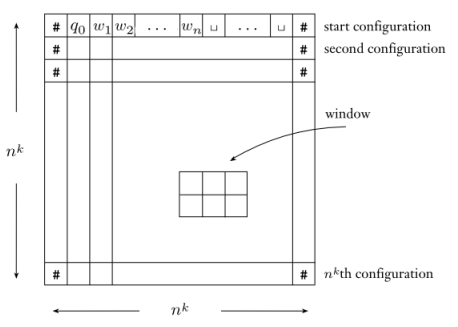
\includegraphics[width=0.6\textwidth]{images/tableau-coock-levin.PNG}
    %\captionof{figure}{}
\end{minipage}

Per convenienza nel seguito assumiamo che ciascuna configurazione inizi e finisca con un simbolo \#. Pertanto, la prima e l'ultima colonna di un tableau sono tutti \#. La prima riga di un tableau è la configurazione iniziale di $N$ su $w$, e ciascuna riga segue dalla precedente in accordo alla funzione di transizione di $N$. Un tableau è accettante se qualche riga del tableau è una configurazione accettante.

Ogni tableau accettante per $N$ su $w$ corrisponde ad una diramazione della computazione accettante di $N$ su $w$. Quindi, il problema di stabilire se $N$ accetta $w$ è equivalente al problema di stabilire se esiste un tableau accettante per $N$ su $w$.

Passiamo ora alla descrizione della riduzione di tempo polinomiale $f$ di $A$ a $SAT$. Su input $w$, la riduzione produce una formula $\phi$. Iniziamo descrivendo le variabili di $\phi$. Siano $Q$ e $\Gamma$ l'insieme degli stati e l'alfabeto del nastro di $N$, rispettivamente. Sia $C = Q\cup\Gamma\cup\{\#\}$. Per ciascun $i$ e $j$ tra 1 ed $n^k$ e per ciascun $s$ in $C$, introduciamo una variabile, $x_{i,j,s}$.

Ciascuna delle $(n ^ k) ^ 2$ entrate di un tableau è chiamata cella. La cella in riga $i$ e colonna $j$ viene denotata con $cell[i, j]$ e contiene un simbolo di $C$. Rappresentiamo i contenuti delle celle con le variabili di $\phi$. Se $x_{i,j,s}$ assume il valore 1, significa che $cell[i, j]$ contiene $s$.

Progettiamo a questo punto $\phi$ in modo tale che un assegnamento che soddisfa le variabili di $\phi$ corrisponda ad un tableau accettante per $N$ su $w$. La formula $\phi$ è l'AND di quattro parti: $\phi_{cell}\land\phi_{start}\land\phi_{move}\land\phi_{accept}$. Descriviamo ciascuna parte, una per volta.

Come anticipato precedentemente, porre a 1 la variabile $x_{i,j,s}$ corrisponde a posizionare il simbolo $s$ in $cell[i, j]$. La prima cosa che dobbiamo garantire al fine di ottenere una corrispondenza tra un assegnamento ed un tableau è che l'assegnamento ponga ad 1 esattamente una variabile per ciascuna cella. La formula $\phi_{cell}$ garantisce questo requisito esprimendolo in termini di operazioni booleane: 
\begin{equation*}
\phi_{cell} = \bigwedge_{1\leq i ,j\leq n^k} \left[\left(\bigvee_{s\in C} x_{i,j,s}\right)\land\left(\bigwedge_{s,t\in C, s\neq l} (\overline{x_{i,j,s}}\lor\overline{x_{i,j,s}})\right)\right]
\end{equation*}
I simbolie $\bigwedge$ e $\bigvee$ stanno per AND ed OR iterati. Per esempio, l'espressione nella formula precedente è un'abbreviazione per 
\begin{equation*}
    \bigvee_{s\in C}x_{i,j,s}
\end{equation*}
è un'abbreviazione per
\begin{equation*}
    x_{i,j,s_1}\lor x_{i,j,s_2} \lor...\lor x_{i,j,s_l}
\end{equation*}
dove $C=\{s_1, s_2, ..., s_l\}$. Quindi, $\phi_{cell}$ è in realtà un'espressione grande che contiene un frammento per ciascuna cella nel tableau, poiché $i$ e $j$ variano da 1 a $n ^ k$. La prima parte del frammento stabilisce che almeno una variabile assume valore 1 nella cella corrispondente. La seconda parte di ciascun frammento stabilisce che non più di una variabile assume valore 1 (letteralmente, stabilisce che, in ogni coppia di variabili, almeno una assume valore 0) nella cella corrispondente. Questi frammenti sono collegati attraverso operazioni $\land$.

La prima parte di $\phi_{cell}$ all'interno delle parentesi garantisce che almeno una variabile che è associata con ciascuna cella vale 1, laddove la seconda parte garantisce che non più di una variabile vale 1 per ciascuna cella. Qualsiasi assegnamento alle variabili che soddisfa $\phi$ (e di conseguenza $\phi_{cell}$) deve avere esattamente una variabile ad 1 per ogni cella. Pertanto, qualsiasi assegnamento che soddisfa $\phi$ specifica un simbolo in ciascuna cella della tabella. Le parti $\phi_{start}$, $\phi_{move}$, e $\phi_{accept}$ garantiscono che questi simboli corrispondano realmente ad un tableau accettante come segue.

La formula $\phi_{start}$ assicura che la prima riga della tabella sia la configurazione iniziale di $N$ su $w$, richiedendo esplicitamente che le variabili corrispondenti siano ad 1:
\begin{equation*}
    \phi_{start} =x_{1, 1, \#}\land x_{1,2,q_0}\land x_{1, 3, w_{1}}\land x_{1,4,w_2}\land ...\land x_{1,n+2,w_n}\land x_{1,n+3,\sqcup}\land...\land x_{1,n^k-1,\sqcup}\land x_{1,n^k,\#}
\end{equation*}

La formula $\phi_{accept}$ garantisce che una configurazione accettante sia presente nel tableau. Essa assicura che $q_{accept}$, il simbolo per lo stato di accettazione, compaia in una delle celle del tableau, richiedendo che una delle variabili corrispondenti sia a 1:
\begin{equation*}
    \phi_{accept} = \bigvee_{1\leq i, j\leq n^k} x_{i,j,q_{accept}}
\end{equation*}

Infine, la formula $\phi_{move}$ garantisce che ciascuna riga del tableau corrisponda ad una configurazione che segue legittimamente dalla configurazione della riga precedente, in accordo alle regole di $N$. Lo fa assicurando che ogni finestra di celle $2\times 3$ sia lecita. Diciamo che una finestra $2\times 3$ è lecita se non viola le azioni specificate dalla funzione di transizione di $N$. In altre parole, una finestra è lecita se può esser presente quando una configurazione segue correttamente da un'altra.

\begin{minipage}{\textwidth}
    \centering
    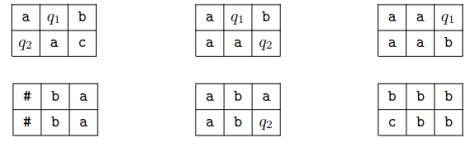
\includegraphics[width=0.6\textwidth]{images/finestre-lecite.PNG}
    %\captionof{figure}{}
\end{minipage}

Le finestre (a) e (b) sono lecite perché la funzione di transizione permette ad $N$ di muovere nella direzione indicata. La finestra (c) è lecita perché, con $q_1$ presente sul lato destro della riga di sopra, non sappiamo su quale simbolo la testina sia. Detto simbolo potrebbe essere una $a$, e $q_1$ potrebbe cambiarlo in una be muovere a destra. Una tale possibilità genererebbe questa finestra, quindi essa non viola le regole di $N$. La finestra (d) è ovviamente lecita perché la riga di sopra e quella di sotto sono identiche, situazione che si verifica se la testina non è adiacente alla posizione della finestra. Si noti che \# in una finestra lecita può comparire a sinistra o a destra sia nella riga superiore che in quella inferiore. La finestra (e) è lecita perché lo stato $q_1$ potrebbe essere immediatamente a destra della riga superiore e la macchina, leggendo una b, si sarebbe mossa a sinistra nello stato $q_2$ che ora compare all'estremità destra della riga inferiore. Infine, la finestra (f) è lecita perché lo stato $q_1$ potrebbe essere stato immediatamente a sinistra della riga superiore, e la macchina potrebbe aver cambiato la $b$ in una $c$ ed effettuato una mossa a sinistra.

\begin{minipage}{\textwidth}
    \centering
    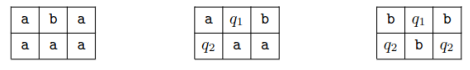
\includegraphics[width=0.6\textwidth]{images/finestre-non-lecite.PNG}
    %\captionof{figure}{}
\end{minipage}

Nella finestra (a), il simbolo centrale nella riga superiore non può cambiare perché non c'è uno stato ad esso adiacente. La finestra (b) non è lecita perché la funzione di transizione specifica che la $b$ viene cambiata in una $c$ ma non in una $a$. La finestra (c) non è lecita perché due stati compaiono nella riga inferiore.

Se la riga superiore del tableau è la configurazione iniziale ed ogni finestra nel tableau è lecita, ciascuna riga del tableau è una configurazione che segue legittimamente dalla precedente.

Proviamo l'asserto considerando ogni coppia di configurazioni adiacenti nel tableau, indicate come la configurazione superiore e la configurazione inferiore. Nella configurazione superiore, ogni cella che contiene un simbolo di nastro e non è adiacente ad un simbolo di stato rappresenta la cella centrale superiore in una finestra in cui la riga superiore non contiene stati. Pertanto, questo stesso simbolo deve comparire al centro in basso nella finestra. Quindi, esso è presente nella stessa posizione nella configurazione inferiore.

La finestra contenente il simbolo di stato nella cella centrale superiore garantisce che le tre posizioni corrispondenti vengano aggiornate consistentemente tramite la funzione di transizione. Pertanto, se la configurazione superiore è una configurazione lecita, altrettanto lo è la configurazione inferiore, e quella inferiore discende da quella superiore in accordo alle regole di $N$.

Torniamo ora alla costruzione di $\phi_{move}$. Essa garantisce che tutte le finestre nel tableau sono lecite. Ciascuna finestra contiene sei celle, che possono essere impostate in un numero fissato di modi per produrre una finestra lecita. La formula $\phi_{move}$ stabilisce che le impostazioni delle sei celle devono essere uno di questi modi, ossia
\begin{equation*}
    \phi_{move} = \bigwedge_{1\leq i < n^k, 1<j<n^k} \textit{(la finestra }(i,j)\textit{ è lecita)}
\end{equation*}

La finestra $(i, j)$ ha $cell[i, j]$ in posizione centrale in alto. Sostituiamo il testo "la finestra $(i, j)$ è lecita" in questa formula con la formula seguente. Denotiamo il contenuto delle sei celle di una finestra con $a_{1} ,...,a_6$.
\begin{equation*}
    V (x_{i,j-1,a_{1}}\land x_{i,j,a_2}\land x_{i,j+1,a_3}\land x_{i+1,j-1,a_4}\land x_{i+1,j,a_5}\land x_{i+1,j+1,a_6})   
\end{equation*}

Nel seguito analizziamo la complessità della riduzione per mostrare che essa opera in tempo polinomiale. Per far ciò, esaminiamo la dimensione di $\phi$. Prima di tutto, stimiamo il numero di variabili che ha. Si ricordi che il tableau è una tabella $n ^ k \times n ^ k$ quindi contiene $n ^{2k}$ celle. Ciascuna cella ha $l$ variabili associate ad essa, dove $l$ è il numero di simboli in $C$. Poiché $l$ dipende soltanto dalla TM $N$ e non dalla lunghezza dell'input $n$, il numero totale di variabili è $O(n^{2k})$.

Stimiamo la dimensione di ciascuna delle parti di $\phi$. La formula $\phi_{cell}$ contiene un frammento di dimensione fissata della formula per ciascuna cella del tableau, quindi la sua dimensione è $O(n^{2k})$. La formula $\phi_{start}$ ha un frammento per ciascuna cella nella riga superiore, quindi la sua dimensione è $O(n ^ k)$. Le formule $\phi_{move}$ e $\phi_{accept}$ contengono ciascuna un frammento di dimensione fissata della formula per ciascuna cella del tableau, quindi la loro dimensione è $O(n^{2k})$. Pertanto, la dimensione complessiva di $\phi$ è $O(n^{2k})$.
\end{demonstration}
\end{Thm}

\subsection{Classi coP, coNP e coEXP}
\begin{Definition}{Classi $coP$, $coNP$ e $coEXP$}{}
Definiamo le classi dei linguaggi $coP$, $coNP$ e $coEXP$ come:
\begin{align*}
coP &= \{A\in DEC | \overline{A}\in P\}\\
coNP &= \{A\in DEC | \overline{A}\in NP\}\\
coEXP &= \{A\in DEC | \overline{A}\in EXP\}
\end{align*}
\end{Definition}

\begin{Thm}{Chiusura del complemento di $P$}{}\label{thm:chiusura-comp-P}
Date le classi $P$ e $coP$, si ha che:
\begin{equation*}
    P = coP    
\end{equation*}
In altre parole, la classe $P$ è chiusa nel complemento.
\begin{demonstration}
Analizziamo la prima implicazione. Dato $A\in P$, sia $D$ il decisore polinomiale tale che $L(D) = A$. Sia $D$ la TM definita come:

$D =$ "Data la stringa w in input:
\begin{enumerate}
    \item Esegui il programma di $D$ su input $w$
    \item Se l’esecuzione accetta, rifiuta. Altrimenti, accetta"
\end{enumerate}
Per costruzione stessa di $\overline{D}$, abbiamo che:
\begin{equation*}
    x\in L(\overline{D})\iff x\notin L(D) = A
\end{equation*}
implicando che $L(\overline{D}) = \overline{A}$. Inoltre, poiché $D$ è un decisore polinomiale, ne segue che anche $\overline{D}$ lo sia, concludendo che $\overline{A} = L(\overline{D})\in P$ e dunque che $A\in coP$.

La seconda implicazione è analoga alla prima.
\end{demonstration}
\end{Thm}

\begin{Thm}{Chiusura del complemento di $EXP$}{}
Date le classi $EXP$ e $coEXP$, si ha che:
\begin{equation*}
    EXP = coEXP    
\end{equation*}
In altre parole, la classe $EXP$ è chiusa nel complemento. 

La dimostrazione è analoga al Teorema \ref{thm:chiusura-comp-P}.
\end{Thm}

\begin{Corollario}{$P\subseteq coNP\subseteq EXP$}{}
Date le classi $P$, $coNP$ e $EXP$, si ha che:
\begin{equation*}
    P\subseteq coNP\subseteq EXP    
\end{equation*}
\begin{demonstration}
Dato $A\in P$, per i Teoremi \ref{cor:gerarchia-temp-ling} e \ref{thm:chiusura-comp-P}, abbiamo che:
\begin{itemize}
    \item $A\in P\implies A\in P\subseteq NP\implies A\in coNP$
    \item $A\in coNP\implies A\in NP\subseteq EXP\implies A\in EXP$
\end{itemize}
implicando che $P\subseteq coNP\subseteq EXP$.    
\end{demonstration}

\begin{minipage}{\textwidth}
    \centering
    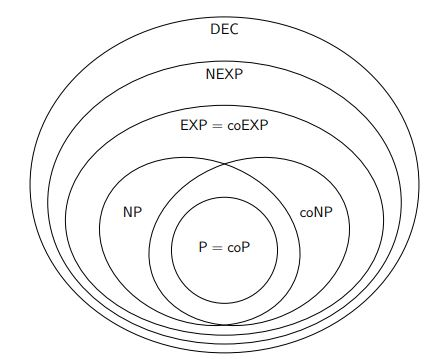
\includegraphics[width=0.5\textwidth]{images/gerarchia-classe-linguaggi.JPG}
    %\captionof{figure}{}
\end{minipage}
\end{Corollario}

\begin{Thm}{$P = NP\implies P = coNP$}{}\label{thm:p=npimpliesp=conp}
Date le classi $P$, $NP$ e $coNP$, si ha che:
\begin{equation*}
    P = NP\implies P = coNP    
\end{equation*}
\begin{demonstration}
Per il corollario precedente, sappiamo che $P\subseteq coNP$. Dato $A\in coNP$, per l’ipotesi e per il Teorema \ref{thm:chiusura-comp-P}, si ha
che:
\begin{equation*}
    A\in coNP\implies A\in NP = P\implies A\in P    
\end{equation*}
concludendo quindi che $P = coNP$.
\end{demonstration}
\end{Thm}

\begin{Corollario}{$NP\neq coNP\implies P\neq NP$}{}
Date le classi $P$, $NP$ e $coNP$, si ha che:
\begin{equation*}
    NP\neq coNP\implies P\neq NP
\end{equation*}
\begin{demonstration}
Tramite il Teorema \ref{thm:p=npimpliesp=conp}, si ha che:
\begin{equation*}
    P = NP\implies P = coNP\implies coNP = NP    
\end{equation*}
Dunque, per contronominale, otteniamo che:
\begin{equation*}
    NP\neq coNP\implies P\neq NP    
\end{equation*}
\end{demonstration}
\end{Corollario}

\begin{Definition}{Classe $coNP-Complete$}{}
Definiamo la classe dei linguaggi $coNP-Completi$ come:
\begin{equation*}
    coNP-Complete = \{L\in DEC | L\textit{ è }coNP-Completo\}
\end{equation*}
dove un linguaggio $B$ è detto $coNP-Completo$ se:
\begin{itemize}
    \item $B\in coNP$
    \item $\forall A\in coNP$ $A\leq^P_mB$
\end{itemize}
\end{Definition}

\begin{Thm}{Completezza del complemento in NP-Complete}{}\label{thm:completezza-com-np-complete}
Dato un linguaggio $B$ si ha che:
\begin{equation*}
    B\in NP-Complete\iff B\in coNP-Complete    
\end{equation*}
\begin{demonstration}
Si ha che:
\begin{align*}
    B\in NP-Complete\iff B\in NP, \forall A\in NP A\leq^P_m B\iff B\in NP, \forall A\in NP A\leq^P_m B\iff\\ B\in coNP, \forall A\in coNP A\leq^P_m B\iff B\in coNP-Complete
\end{align*}    
\end{demonstration}
\end{Thm}

\begin{Thm}{Uguaglianza tra $NP$ e $coNP$}{}\label{thm:uguaglianza-np-conp}
Dato un linguaggio $B\in NP-Complete$, si ha che:
\begin{equation*}
    B\in coNP\iff NP = coNP    
\end{equation*}
\begin{demonstration}
Analizziamo la prima implicazione. Poiché $B\in coNP\iff B\in NP$ e poiché $B\in NP-Complete$, si ha che:
\begin{equation*}
    A\in NP\implies A \leq^P_m B\iff A \leq^P_m B\implies A\in NP\iff A\in coNP    
\end{equation*}
implicando che $coNP\subseteq NP$. Viceversa, si ha che:
\begin{equation*}
    A\in coNP\implies A\in NP\implies A\leq^P_m B\implies A\in NP    
\end{equation*}
implicando che $NP\subseteq coNP$.

Per la seconda implicazione. Se $NP = coNP$, allora $B\in NP-Complete\subseteq NP = coNP$.
\end{demonstration}
\end{Thm}

\begin{Definition}{Problema dell’insoddisfacibilità}{}
Definiamo il linguaggio del problema dell’insoddisfacibilità come:
\begin{equation*}
    UNSAT = \{\langle\emptyset\rangle | \emptyset\textit{ è una formula insoddisfacibile}\}
\end{equation*}
\end{Definition}

\begin{Thm}{$coNP$-Completezza di $UNSAT$}{}
\textit{Dato il linguaggio $UNSAT$, si ha che $UNSAT\in coNP-Complete$.}
\begin{demonstration}
Per il Teorema di Cook-Levin sappiamo che $SAT$ sia $NP-Completo$. Di conseguenza,
per il Teorema \ref{thm:completezza-com-np-complete} sappiamo che $\overline{SAT}$ sia $coNPCompleto$.

Sia quindi $f : \Sigma^*\to \Sigma^*$ la funzione calcolata dalla seguente TM $F$:

$F =$ "Data la stringa $x$ in input:
\begin{enumerate}
    \item Verifica se $x = \langle\emptyset\rangle$ per qualche formula $\emptyset$.
    \item Se vero, restituisci $x$. Se falso, restituisci la stringa $\langle a\land \lnot a\rangle$"
\end{enumerate}
Notiamo che se $x\notin \overline{SAT}$ allora $x\in SAT$ e dunque sicuramente $x = \langle\emptyset\rangle$ per qualche formula soddisfacibile $\emptyset$, implicando che $f(x) = \langle\emptyset\rangle\notin UNSAT$. Invece, se $x\in \overline{SAT}$ allora abbiamo due opzioni:
\begin{itemize}
    \item Se $x\in \overline{SAT}$ in quanto $x$ è non è una formula valida allora $f(x) = \langle a \land \lnot a\rangle\in UNSAT$ in quanto la formula $a\land \lnot a$ è insoddisfacibile.
    \item Se $x\in \overline{SAT}$ in quanto $x$ è una formula valida allora $f(x) = \langle\emptyset\rangle\in UNSAT$ in quanto la formula $\emptyset$ è insoddisfacibile.
\end{itemize}
Ciò conclude che $x\in \overline{SAT}\iff f(x)\in UNSAT$. Inoltre, la macchina $F$ richiede tempo polinomiale, concludendo che $\overline{SAT}\leq^P:m UNSAT$. Infine, poiché $\overline{SAT}$ è $coNP-Completo$ ed è riducibile a $UNSAT$, concludiamo che anche $UNSAT$ sia
$coNP-Completo$.
\end{demonstration}
\end{Thm}